\section{Wavelet-based Diffusion Pipeline}

The diffusion model presented in Chapter~3 operates directly on the density
fields in physical space. While this setting already provides a meaningful
baseline, it does not explicitly exploit the multi-scale structure discussed in
Chapter~2. Rayleigh--Taylor instability fields contain both large coherent
structures and fine localized fluctuations, and these components are not
equally easy to learn in pixel space. In particular, the small-scale features
associated with interface corrugations, local mixing events, and turbulent
details can be difficult to preserve when the model must simultaneously learn
the global morphology of the flow.

This observation motivates a second generative pipeline based on wavelet
coefficients. The main idea is to decompose each density field into an
approximation component, which captures the large-scale structure, and detail
components, which encode the local variations at a given resolution level. A
diffusion model is then trained not on the raw image itself, but on this
multi-resolution representation. The resulting surrogate is expected to better
capture the hierarchical organization of RTI fields and to produce samples that
preserve the dominant scales of the flow while remaining flexible enough to
reconstruct realistic fine-scale structures.

Compared with the baseline diffusion model, this approach introduces an
additional inductive bias: instead of learning the full spatial field at once,
the network learns to generate the wavelet detail coefficients conditioned on
the coarse approximation. 

An important difference also appears at the level of the prior. In the direct
diffusion model, generation starts from pure Gaussian noise having the same
spatial size as the target image. In the wavelet setting, the initial noise is
defined in coefficient space and is therefore smaller by a factor related to
the decomposition level $j$. In practice, a wavelet decomposition reduces the
resolution of the latent variable by approximately $2^j$ in each spatial
direction, so the generative model begins from a more compact prior while
still preserving the hierarchical structure needed to reconstruct the full
field.
This direct-versus-wavelet organization is summarized in
Figure~\ref{fig:ch5_wavelet_diffusion_scheme}.

\begin{figure}[H]
    \centering
    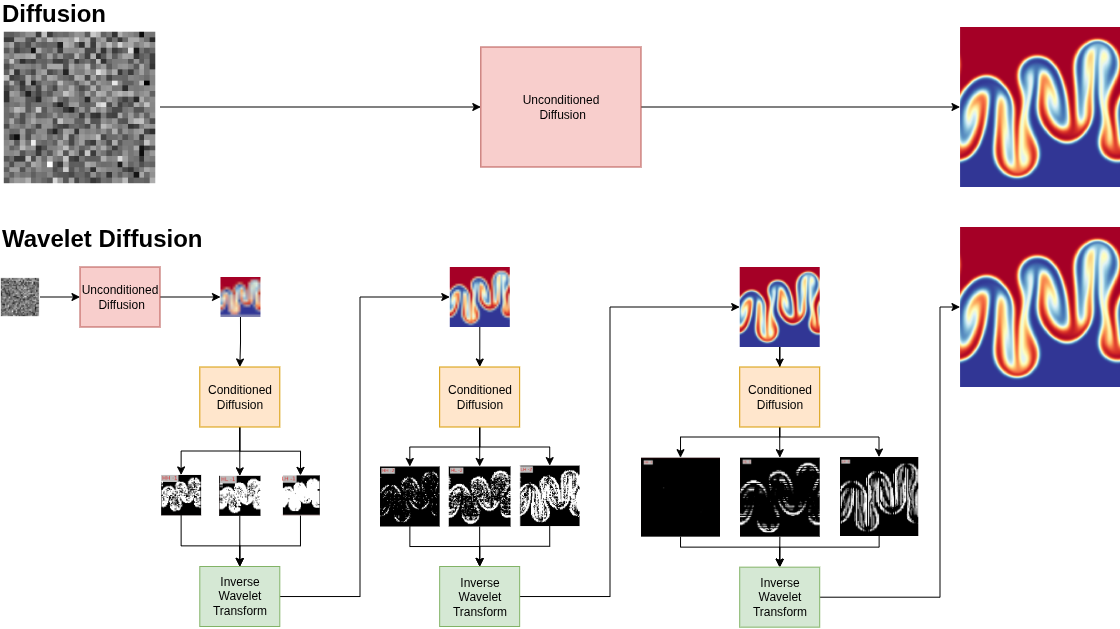
\includegraphics[width=0.95\textwidth]{figures/ch5/WaveletDiffusion.png}
    \caption{Comparison between direct diffusion and wavelet-based diffusion. In the wavelet case, the prior is defined on a lower-resolution latent representation before the inverse wavelet transform reconstructs the full field.}
    \label{fig:ch5_wavelet_diffusion_scheme}
\end{figure}



